
\chapter{Audit}

Audit viene dal latino \textit{audere}, ovvero ascoltare.


Indagine forense, cerca recuperare informazioni dai sistemi informatici, ora è 
difficile per via del cloud.





\paragraph*{Definizione}

Un processo sistematico nel quale un team qualificato, competente e indipendente 
ottiene in maniera obiettiva\footnote{La \textit{Evidence} significa prova, e 
tutti i sentimenti del tipo ``ho sentito che'' non sono prove, e per questo non 
possono far parte dell'audit.} e valutano le asserzioni riguardo ai processi con 
l'obiettivo di creare un'opinione a riguardo e riportare il grado in cui 
l'asserzione è implementata.


\section{Qualità di un Auditor}

L'auditor deve avere le seguenti qualifiche:
\begin{itemize}
\item Indipendenza professionale: 
\item Indipendenza organizzativa: 
Auditor non deve avere interessi o dipendenze gerarchiche con l'unità aziendale 
sotto audit. L'auditor sta sotto il diretto controllo del CEO. Perchè non può 
auiditare qualcuno che sta sopra nella scala gerarchica perchè potrebbe essere 
influenzato dal suo ruolo subordinato.
\end{itemize}


L'auditor è in un processo di formazione continua. Per esempio certificazioni 
richiedono continui aggiornamenti dal punto di vista professionale.







\section{IS Audit Definition}

La prima attività che fa l'auditor è guadagnare la comprensione del soggetto che 
sta analizzando (es. contesto aziendale).
La seconda è valutare i controlli e l'ultima è testare i controlli, come mostrato nella figura \ref{fig:is:audit:definition}.


Cerca di capire il contesto aziendale, dove sta accendo e le relazioni tra le 
unità aziendali. Cerca di prendere contatto con la realtà aziendale che lo 
circonda.


\begin{figure}[h!]
	\begin{center}
		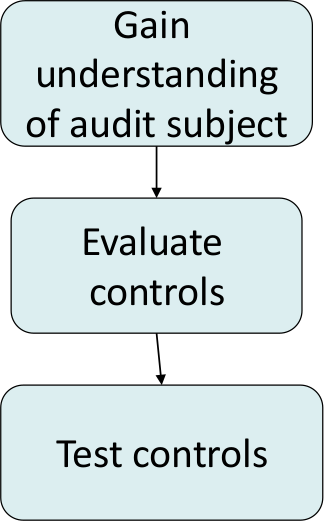
\includegraphics[scale=0.4]{res/img/is_audit_definition.png}
	\end{center}
	\caption{Diagramma di flusso (semplificato) per il processo di IS audit.}
	\label{fig:is:audit:definition}
\end{figure}

\section{Pianificazione dell'audit}

Attualmente la pianificazione dell'audit viene fatta ogni 3 anni.
Esistono due tipologie di Audit:
\begin{enumerate}
\item Breve termine 
\item Lungo termine

\end{enumerate}

È importante durante un audit porsi delle domande per poter porre correttamente 
il lavoro a termine.
Cosa testiamo per prima?
\begin{itemize}
\item Qual è la parte del nostro business più sensibile al rischio?
\item I sistemi sono soggetti a cambiamento?
\item Che regole dobbiamo testare?
\item Ci sono nuove regole da testare?
\end{itemize}


L'audit è molto importante soprattutto in zone definite come critiche. Zone di 
guerra sono spesso soggette a corruzione, e quindi il lavoro di audit risulta 
essere difficile da eseguire.

\todo{Inserire tabella di esempio(?)}

\section{Procedura estesa di audit}

Come già detto, è importante capire la realtà in cui ci si trova. È poi 
fondamentale eseguire un \textit{risk assessment} per capire le zone di rischio 
maggiore.
Infine viene preparato il piano, in cui verranno controllate diverse aree. 
Vengono esaminati anche lavori precedenti, con la revisione della documentazione 
e vengono eseguite interviste. Le interviste sono molto importanti perchè 
permettono, con le giuste domande, di acquisire molte informazioni.
I \textit{test di compliance} eseguono i controlli sulla corretta esecuzione dei 
test.

Viene poi steso il rapporto di Audit, a cui a seguire ci sono delle attività 
secondarie. Queste attività secondarie dipendono da che tipo di Audit è:
\begin{itemize}
\item Esterno: queste attività di solito non vengonono eseguite
\item Interno: queste attività vengono continuate
\end{itemize}

La consegna dell'Audit implica una interazione con chi non gestisce 
correttamente un determinato processo: è infatti importante non solamente 
consegnare l'Audit ma anche discutere dei problemi presenti per poter migliorare 
la situazione.

\section{Esecuzione di un audit}

\subsection{Step 1: Ottenere la comprensione dell'area soggetta ad audit}

Questa è la fase iniziale, che comprende differenti passi che devono essere 
eseguiti sistematicamente.
Questi passi sono:
\begin{itemize} 
\item Tour delle strutture relative all'audit
\item Lettura dei documenti (es. risk assessment, documenti di processi andati 
male)
\item Revisione del piano di business e del piano IT strategico
\item Interviste alle persone chiave per capire il business dell'azienda.
\item Lettura degli audit precedenti
\item Capire qual è la regolamentazione da applicare
\item Identificare le aree che sono state esternalizzate
\end{itemize}

\subsection{Step 2: Perform risk assessment} 

Questi termini sono molto importanti\footnote{Chiesti all'esame dal prof.}

\paragraph*{Rischio inerente}

È il rischio legato all'attività che viene svolta\footnote{Legato al business.} 
(es. per una fabbrica di fuochi di artificio il rischio inerente è 
l'esplosione).

Per esempio, per una farmacia, il rischio inerente è:
\begin{itemize}
\item Truffa
\item Rapina
\end{itemize}

\paragraph*{Rischio di controllo}

Un rischio che non può essere rilevato da un controllo interno. Ovvero un 
rischio che possa passare inosservato.

L'auditor trova un problema che non esista. È possibile che venga trovato un 
problema che non esista.


\paragraph*{Rischio della detection}

Un auditor non riesche a rilevare un problema che esiste. Per esempio nel caso di una banca avviene una frode che non viene detectata.


% La traduzione non è perfetta penso:(
\paragraph*{Rischio generale dell'Audit}

Che sono i rischi detti precedentemente (una sua combinazione).



\subsection{Step 3: Preparare un piano di Audit}

È importante prendere un lavoro di Audit che sia pianificabile in tempo: 
prendere lavori che devono essere svolti in pochissimo tempo non sono fruttuosi, 
in quanto il lavoro viene eseguito solitamente male e si ha di ritorno una 
cattiva pubblicità. In questo segmento di mercato, farsi una buona reputazione 
ci si mette tanto tempo, mentre per rovinarsela ci vuole pochissimo. Quindi se 
si vede che non c'è abbastanza tempo per eseguire quel determinato lavoro è 
meglio non eseguirlo. 
È importante avere anche i giusti spazi: la disponibilità della segreterie per 
eseguire fotocopie di documenti per esempio\footnote{Solitamente, questa cosa 
vale in base all'NDA firmato.} migliora di sicuro la qualità del lavoro svolto 
(questo vale anche, per esempio, per avere un piccolo spazio/ufficio su cui 
eseguire l'Audit). Per i documenti non cartacei, coem quelli elettronici, devono 
essere rilasciate garanzie su dove vengono salvati, come ad esempio se è 
presente la cifratura sul dispositivo di storicizzazione o meno.

L'Audit si sviluppa un approccio basato sul rischio e vengono inclusi obiettivi, 
scopo, tempo e risorse richieste per l'audit.

La pianificazione dev'essere eseguita correttamente, in quanto solitamente i 
tempi per eseguire un Audit non è molto e sono presenti \textit{deadline} 
strette.




\subsubsection{Vocabolario della Pianificazione dell'Audit}

In una pianificazione dell'audit, sono importanti tenere a mente i seguenti 
vocaboli:
\begin{itemize}
\item Audit subject: l'area che viene auditata
\item Obiettivo dell'audit: lo scopo dell'audit (es. determinare se un processo 
è controllato bene)
\item Contesto dell'audit: limitare l'audit ad uno specifico sistema, funzione, 
oggetto.
\end{itemize}

\paragraph*{Esempio}

\begin{figure}[h!]
	\begin{center}
		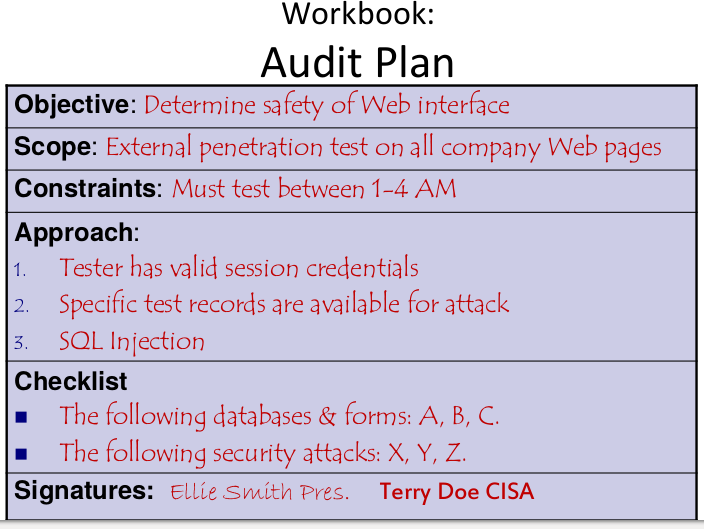
\includegraphics[scale=0.4]{res/img/audit_plan_vocabulary_example.png}
	\end{center}
	\caption{Esempio per prendere confidenza con i termini dell'audit plan.}
	\label{fig:audit:plan:vocabulary:example}
\end{figure}






\subsection{Step 4: Aggiungere dettagli al piano}


Tradurre gli oggetti dell'audit in oggetti più specifici.

Identificare e selezionare l'approccio di audit per testare e verificare i 
controlli.

Identificare gli individui da intervistare

Ottenere le policy, standardn procedure e linee guida aziendali.

\todo{Da completare}

\subsection{Step 5: Valutare l'area di audit}

Vengono usati \textit{tool} di tipo generale, e anche osservazioni sul campo. 
Queste osservazioni sul campo sono sempre molto utili, perchè permette di vedere 
effettivamente come i dipendenti stanno lavorando (per esempio osservando un 
amministratore di sistema si potrebbe scoprire se è stata applicata una corretta 
\textit{segregation of duties}), e permette di scoprire elevate criticità.


\todo{step 5 o 6?}
È sempre molto importante lavorare sulla struttura organizzativa, che devono 
essere aggiornate in maniera continua.
Altri punti importanti:
\begin{itemize}
\item Review IS organization: separation of duties
\item Revisione delle policy, standard, procedure di IS: definite, aggiornate 
periodicamente. Sulle policy viene indicato il versionamento del documento 
(versione, data, firma di chi ha autorizzato).
\item Revisione della documentazione IS
\item Intervista del personale: segregation of duties, security awareness, 
competenze relative al proprio lavoro. È importante conoscere come i dipendenti 
lavorano all'interno dell'azienda, senza porre domande troppo sospette. Una 
domanda molto importante da fare è: \textit{Come si trova sul lavoro?} In quando 
quando ci si trova a fare dei \textit{task} che non è adatti a fare ci saranno 
molto probabilmente delle difficoltà. Questo da il \textit{sentiment} della 
situazione aziendale.
\item Osservare il personale:\todo{O osservazioni personali?} documentare tutto 
con un livello sufficiente di dettagli, questa documentazione deve essere tale 
da fornire evidenza dei fatti.

\end{itemize}


\subsubsection{Tipologie di controlli}


\begin{itemize}
\item Controlli correttivi: corregge i problemi e previene i problemi futuri
\item Controlli detettivi: servono a rilevare un problema (es. hash totals che 
verifica l'integrità dei file)
\item Controlli preventivi: sono i controlli più difficili da eseguire ma anche 
i migliori perché permettono di evitare il rischio.
\end{itemize}

I \textbf{controlli correttivi} sono quei controlli che risolvono i problemi e 
evitano che quella tipologia di problema risorga nel futuro. Ad esempio il 
\textit{contingency plan}\footnote{Il \textit{contingency plan} è quella 
attività che permette l'erogazione di un servizio anche ad un livello 
degradato.} è uno di questi.

I \textbf{controlli detettivi} controllano per esempio l'integrità delle 
informazioni, come per esempio l'integrità dei database. Esistono software molto 
costosi che permettono di analizzare i log di sistema, per capire maggiori 
informazioni sul sistema.

I \textbf{controlli preventivi} sono i controlli più difficile da eseguire, ma 
quelli che permettono di far risparmiare di più. Alcune cose che solitamente 
sono da verificare sono per esempio che i dischi siano criptati, che il 
personale sia adeguatamente aggiornato e preparato.
Il personale è fondamentale: persone che non sono adatte al ruolo faranno male 
il lavoro, e quindi o verranno/si faranno licenziare subito, causando un elevato 
\textit{turnover}. Questo indice deve essere basso per un'azienda, e costituisce 
un problema enorme in quando prendere una persona costa risorse, in tempo e 
soldi. Questa soglia di \textit{turnover} non deve mai superare la soglia del 
5-7\%.

\subsubsection{Manutenzione dei controlli}
Questi tipi di controlli sono di natura qualitatitva.

Controlli in overlap: va a compensare il rischio di controllo, in modo che se un 
controllo non trova il problema possa trovarlo un altro.

Controllo compensativo: supporta un controllo più debole.

\todo{Copiare tabella}


\subsection{Step 6: Test di Audit}


Evidence: le \textbf{risultanze} (\emph{Findings}) sono basate su prove e fatti 
sufficienti e affidabili e su una corretta interpretazione dell'evidenza. 

La \textbf{documentazione} è fondamentale. Il lavoro di audit e l'evidenza 
dell'audit per supportare le conclusioni devono essere completamente 
documentate.
\todo{RiControlla con le slide}
%Documentazione: il lavoro di audit e l'evidenza dell'audit per supportare le 
conclusioni devono essere completamente documentate. 

La \textbf{supervisione} dev'essere eseguita in maniera professionale, e 
dovrebbe esserci sempre un supervisore o un responsabile.

Lo \textbf{scetticismo} è importante, e ogni azione va guardata con un certo 
occhio di riguardo. Quando si incontrano regolarità bisogna andare in 
profondità, reportando le irregolarità in maniera corretta. Anche le controparti 
vanno informate, e questa tipologie di azioni non vanno eseguite di 
``nascosto''. Lo stesso discorso va fatto anche se la controparte è in malafede.
In caso venga scopera una controparte che è in malafede bisogna avvisare 
immediatamente riguardo alla situazione, perchè è presente il rischio che la 
controparte cancelli le prove che la colpevolizzino.





Supervisione: lo staff di audit viene supervisionato per assicurare che l'audit 
venga eseguito in modo professionale.

Scetticismo professionale: bisognare essere scettici nei confronti dei controlli 
in modo da verificare tutto quello che deve essere verificato.


\subsubsection{Test sostanziali e test di compliance}

Test sostanziali \todo{va troppo veloce}

Test di compliance: c'è qualcosa? Quel qualcosa funziona per quello che è stato 
pensato? Tipicamente viene eseguito tramite una checklist.

Ci sono due tipologie principali di test:
\begin{itemize}
\item Test di complianza, in cui è importante chiedersi: sono i controlli 
presenti eseguiti in maniera consistente?
\item Test sostanziali. Il controllo sostanziale deve sostenere il business. 
%substantive
\end{itemize}


Se i risultati dei test di compliance sono scarsi, mi aspetto che i controlli 
sostanziali siano più numerosi in tipo e numero.

\section{Step 7: Test di compliance}

Controllo: il software in produzione è controllato?
\begin{itemize}
\item Test: I file eseguibili vengono buildati dal codice sorgente che sta nel 
repository? Se questo non accade è un grave problema, perchè significa che si 
sta usando del software in produzione che è diverso da quello che è presente nel 
repository.
\item Test: Sono state seguite le procedure adeguate durante la release? Nelle 
aziende grosse, è presente un libro dei test, in cui chi è responsabile appone 
una firma prima di rilasciare una certa versione del software.
\end{itemize}


\section{Step 8: Test sostanziali}

Audit: is financial statement section related to sales accurate? \todo{tradurre 
appena rallenta}

\begin{itemize}
\item Test: tracciare il processing di un esempio di transazione attraverso il 
sistema, eseguendo i calcoli manualmente
\item Test: testare le condizioni di errore
\end{itemize}



\subsection{Campionamento}

Campionamento statistico: ci sono tecniche standard, fornisce un 
\textit{intervallo di confidenza} (intervallo in cui siamo sicuri che il nostro 
campione sia significativo). Se abbiamo N item, con un campione di $\sqrt{N}$ 
elementi garantisce una precisione del 99.9\%.
$$
(1 - 1/100)^K
$$

Campionamento non stastistico:

Tutto ciò che è statisticamente rappresentato
